\chapter{Histograms Using {\tt matplotlib}}

\setcounter{problem}{1}
\section{Discussion}

\begin{fullwidth}


The goal of this lab is to teach you the basics of using matplotlib to display probability mass functions, otherwise known as histograms. In this lab we will use the uniform distribution. Use filename {\tt hist.py}.

\section{Steps}

\step  import the proper libraries

\begin{pyverbatim}
import matplotlib.pyplot as plt
import numpy as np
\end{pyverbatim}

\step Get a sample of uniform random variables in $U(0,1)$

\begin{pyverbatim}
N = 1000
X = [np.random.uniform(0,1) for i in range(N)] # U(0,1)
# or np.random.uniform(0,1,N)
\end{pyverbatim}

\step Display a histogram using matplotlib (in a separate window)

\begin{pyverbatim}
plt.hist(X, normed=1)
plt.show()
\end{pyverbatim}

\step Run it. \\

\step Now, save the image as a PDF to the same directory by inserting a save command in between the histogram and the show method:

\begin{pyverbatim}
plt.hist(X, normed=1)
plt.savefig('unif-0-1-density.pdf', format="pdf")
plt.show()
\end{pyverbatim}

\step Run it. Your pdf file should look like

\scalebox{.25}{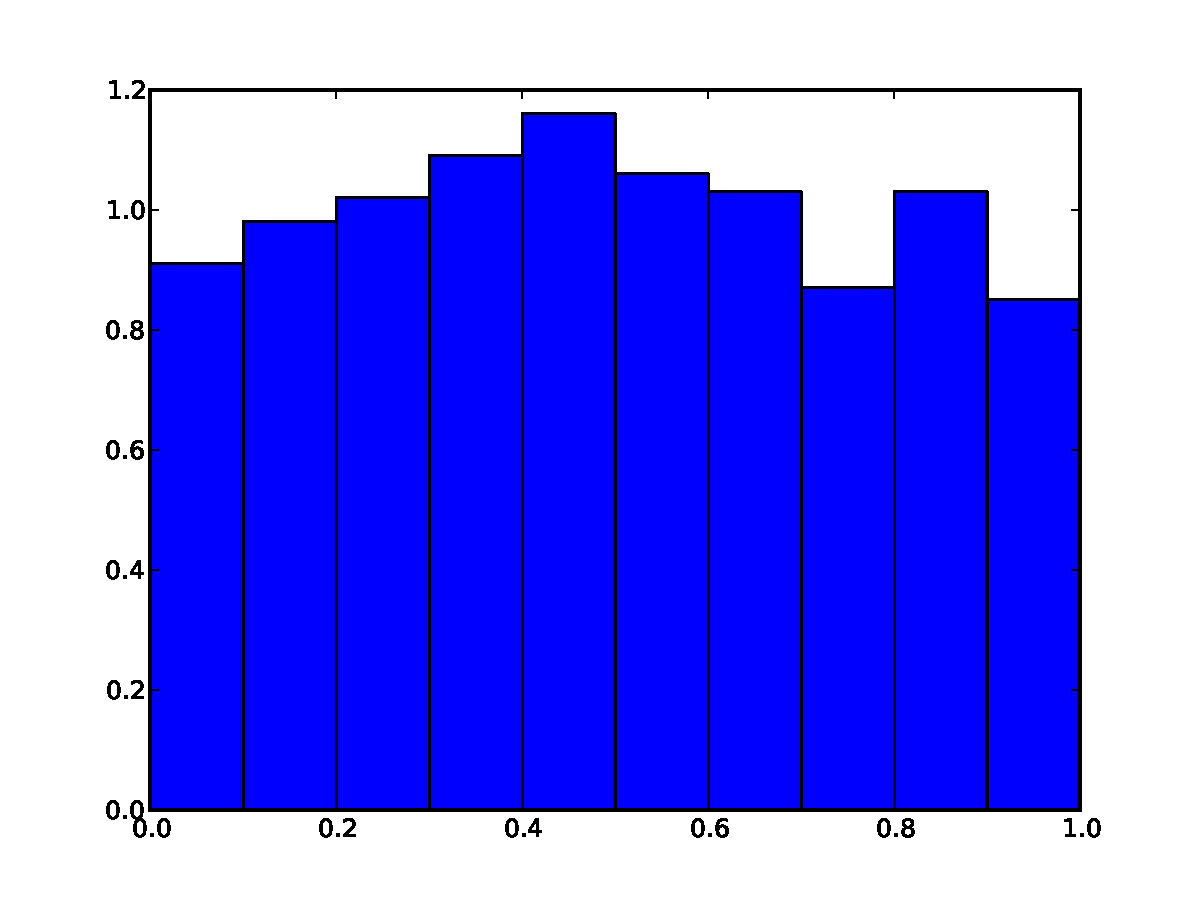
\includegraphics{figures/unif-0-1-density.pdf}}

\step  Graphs should always have the axes labeled. Let's do that as well as add a title and set the range of the graph. Put this code right before the {\tt savefig()}.

\begin{pyverbatim}
plt.title("U(0,1) Density Demo")
plt.xlabel("X", fontsize=16)
plt.ylabel("Density", fontsize=16)
plt.axis([0, 1, 0, 2])
\end{pyverbatim}

\step Run it. \\

\step It's also common to add some annotations inside the graph to explain more about what we are seeing. First, we need to get access to the figure itself and then has to figure about its axes. (We need this in order to specify coordinates within the graph.) Put the following code before the {\tt hist()} call.

\begin{pyverbatim}
fig = plt.figure()        # get a handle on the figure object itself
ax = fig.add_subplot(111) # weird stuff to get the Axes object within figure
\end{pyverbatim}

Then, before the {\tt savefig()},  add the following to display some text above the histogram within the graph. The coordinates are from 0..1 where 0 is the left/bottom edge and 1 is the right/top edge.

\begin{pyverbatim}
# put N=... at top left
plt.text(.1,.9, 'N = %d' % N,
		 fontsize=16,
		 transform = ax.transAxes) 
\end{pyverbatim}

\step Also, let's change the file name slightly so we can keep our original graph plus our fancy one:

\begin{pyverbatim}
plt.savefig('unif-0-1-density-fancy.pdf', format="pdf")
\end{pyverbatim}

\step Run it. \\

\scalebox{.25}{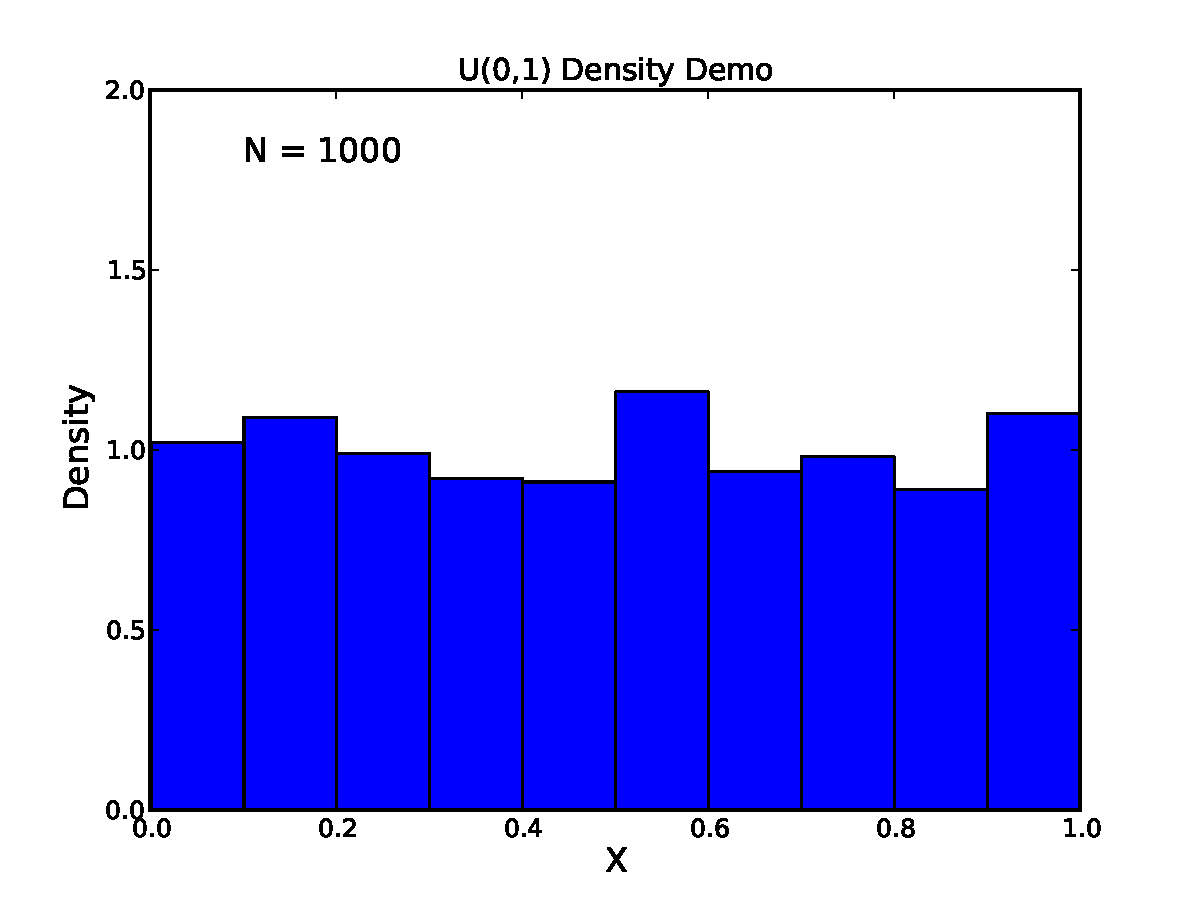
\includegraphics{figures/unif-0-1-density-fancy.pdf}}

{\bf To understand distributions, it's a great idea to start messing around with the parameters of the density or mass function.} \\

\step Change $U(0,1)$ to $U(2,8)$ and examine the results. You will have to alter the axis() to use different ranges. (Or let the plotting software do the work for you and get rid of the axis() call.) Run it. You should see something like the following.

\scalebox{.25}{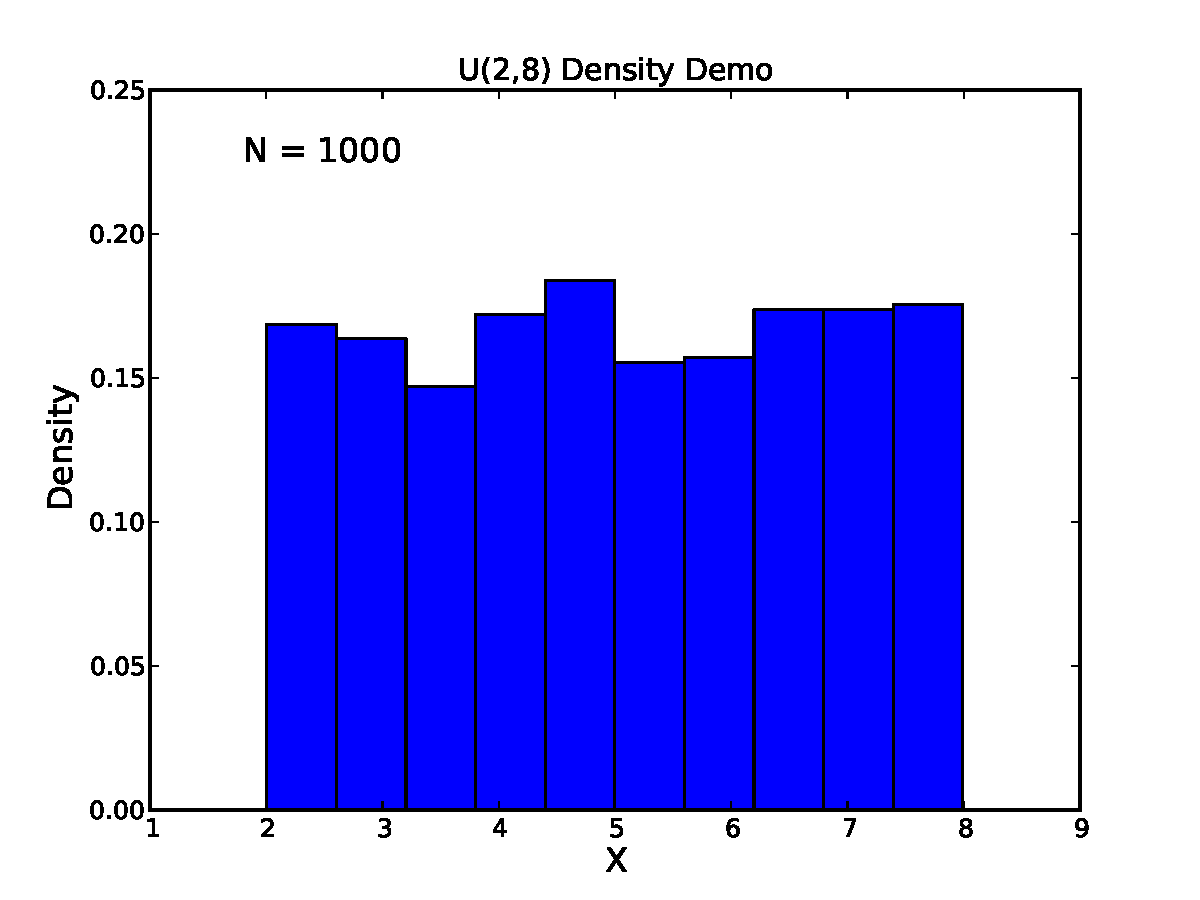
\includegraphics{figures/unif-2-8-density-fancy.pdf}}

\section{Deliverables}

Please submit:

\begin{itemize}
\item your {\tt hist.py} Python file
\item a PDF of your $U(2,8)$ graph.
\end{itemize}

\end{fullwidth}
